\documentclass[10pt]{beamer}

\usetheme{Warsaw}
\beamertemplatenavigationsymbolsempty

\usepackage[utf8]{inputenc}
\usepackage[T1]{fontenc}
\usepackage[francais]{babel}
\usepackage[autolanguage]{numprint}
\renewcommand*{\rmdefault}{fxb}
\usepackage{lettrine}
\usepackage{hyperref}
\usepackage{wasysym}
\usepackage{listings}
\usepackage{xcolor}
\lstset{keywordstyle=\color{blue}, stringstyle=\color{green}}
\usepackage{amsmath}
\usepackage{wrapfig}
\usepackage{euler}
\usepackage{multicol}
\usepackage{graphicx}
\usepackage{tikz}
\usetikzlibrary{mindmap,trees}
\graphicspath{{./img/}}
\DeclareGraphicsExtensions{.png, .jpeg, .jpg}


\renewcommand*\thesection{\arabic{section}}

\AtBeginSection[]{%
  \begin{frame}<beamer>
    \frametitle{Plan}
    \tableofcontents[sectionstyle=show,subsectionstyle=hide]
  \end{frame}
  \addtocounter{framenumber}{-1}
}


\lstset{basicstyle=\footnotesize}

\title{Classification automatique de la fonction de citation}
\author{Rémi Bois et Soufian Salim}
\date{\today}

\begin{document}

\begin{frame}
  \maketitle
\end{frame}

\section{Introduction}
\label{sec:intro}

\begin{frame}
  \frametitle{L'article en question}
  %nom des auteurs, du papier, publication
  
  \begin{block}{Auteurs}
  \begin{itemize}
    \item Simone Teufel, Advaith Siddharthan, Dan Tidhar
    \item Université de Cambridge
    \item NLIP Research Group
  \end{itemize}
  \end{block}

  \begin{block}{Impact}
  \begin{itemize}
    \item Conference on Empirical Methods in NLP - Sydney 2006
    \item 15 citations
  \end{itemize}
  \end{block}
\end{frame}

\begin{frame}
  \frametitle{Pourquoi citons-nous ?}
  %intérêt des citations
  %types de citations (positives, négatives, ...)
  %différence entre fonction et motivation

  \begin{block}{Motivation}
  \begin{itemize}
    \item Propriété subjective
    \item Relation avec l'analyse d'opinion
  \end{itemize}
  \end{block}

  \begin{block}{Fonction}
  \begin{itemize}
    \item Informe sur la relation entre les articles
  \end{itemize}
  \end{block}
\end{frame}

\begin{frame}
  \frametitle{Quel rôle a une citation dans un papier ?}

  \begin{block}{Moravcsik \& Murugesan, 1975}
  \begin{itemize}
    \item Conceptuel / Opérationnel
    \item Évolution / Juxtaposition
    \item Organique / Superficiel
    \item Confirmation / Négation
  \end{itemize}
  \end{block}
\end{frame}

\begin{frame}
  \frametitle{Pourquoi s'intéresser à cette fonction ?}
  %applications au résumé, à la RI via citations, ...
  %motivations (sentiment analisys, ...)
  
  \begin{block}{Approche quantitative insuffisante}
  \begin{itemize}
    \item "Politeness, policy or piety" (Ziman, 1968)
    \item 40\% de citations superficielles
  \end{itemize}
  \end{block}
  
  \begin{block}{Applications}
  \begin{itemize}
    \item Calcul du facteur d'impact
    \item Résumé d'article
    \item RI
  \end{itemize}
  \end{block}
\end{frame}

\begin{frame}
  \frametitle{Application hypothétique}
\begin{figure}[ht!]
\centering
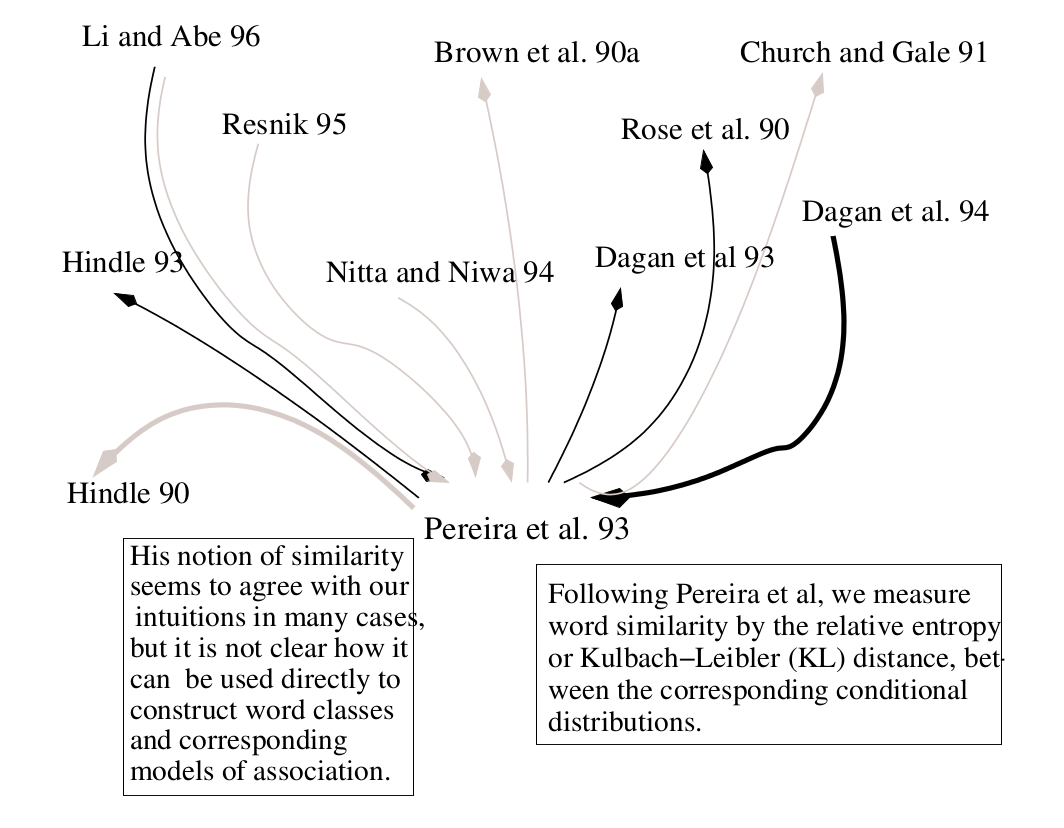
\includegraphics[width=80mm]{citation_map.png}
\caption{Cartographie de citations}
\label{overflow}
\end{figure}

\end{frame}

\begin{frame}
  \frametitle{Objectifs}
  %Objectifs du papier, approche manuelle + apprentissage
  
  \begin{block}{Schéma d'annotations}
  \begin{itemize}
    \item Orienté Faiblesse / Similarité / Contraste
    \item Règles et consignes d'annotation
    \item Traits pertinents pour du ML
  \end{itemize}
  \end{block}
  
  \begin{block}{Expériences}
  \begin{itemize}
  	\item Procéder à une annotation manuelle
    \item Répliquer l'annotation manuelle avec du ML
  \end{itemize}
  \end{block}
\end{frame}

\section{Catégorisation et annotation manuelle}
\label{sec:catandmanual}


\begin{frame}
  \frametitle{Les différentes catégories}
  %tableau des catégories

	\begin{tabular}{| c | c |}
		\hline
		Weak & Critique \\
		\hline
		CoCoGM & Contraste ou comparaison des objectifs ou des méthodes \\
		CoCo- &  Supériorité du travail de l'auteur sur celui cité \\
		CoCoR0 & Contraste ou comparaison des résultats (neutre) \\
		CoCoXY & Contraste ou comparaison entre deux méthodes citées \\
		\hline
		PBas & Basé sur l'article cité \\
		PUse & Utilisation d'éléments de l'article cité \\
		PModi & Adaptation d'éléments de l'article cité \\
		PMot & Motivé par l'article cité \\
		PSim & Similarité entre les travaux \\
		PSup & Compatibilité ou support mutuel entre les travaux \\
		\hline
		Neut & Neutre \\
		\hline
	\end{tabular}
\end{frame}

\begin{frame}
  \frametitle{Les données}
  %source, stats sur la taille des données
  
  \begin{block}{Source}
  \begin{itemize}
    \item Computation and Language E-Print Archive
    \item 360 articles
  \end{itemize}
  \end{block}
  
  \begin{block}{Prétraitement}
  \begin{itemize}
    \item Transformé en XML
    \item Balisage des titres, auteurs et références
    \item Analyse des références, identification des noms d'auteurs
    \item Analyse du texte, identification des références
  \end{itemize}
  \end{block}
\end{frame}

\begin{frame}
  \frametitle{L'annotation manuelle des données}
  %règles, quantités, ...
  
  \begin{block}{}
  \begin{itemize}
    \item 
  \end{itemize}
  \end{block}
  
  \begin{block}{}
  \begin{itemize}
    \item 
  \end{itemize}
  \end{block}
\end{frame}

\begin{frame}
  \frametitle{Résultats de l'annotation manuelle}
  %Kappa, distribution, ...
  
  \begin{block}{}
  \begin{itemize}
    \item 
  \end{itemize}
  \end{block}
  
  \begin{block}{}
  \begin{itemize}
    \item 
  \end{itemize}
  \end{block}
\end{frame}

\section{Classification automatique}
\label{sec:machinelearning}

\begin{frame}
  \frametitle{Du machine learning}
  % KPPV (3), 10-fold
\end{frame}

\begin{frame}
  \frametitle{Les features utilisées}
  %cue phrases, location, ...
\end{frame}

\begin{frame}
  \frametitle{Résultats de la classification automatique}
  %résultats sur les 12 catégories, Kappa, F-measure
\end{frame}

\begin{frame}
  \frametitle{Résultats sur des classes moins nombreuses}
  %tableaux et Kappas sur les 3/4 classes
\end{frame}

\section{Conclusion}
\label{sec:conclusion}

\begin{frame}
  \frametitle{Des premières pistes pour une nouvelle tâche}
  %Premiers résultats "encourageants"
\end{frame}

\begin{frame}
  \frametitle{Quelques limites présentes}
  %Kappa max de 0.72, annotation manuelle très restrictive, ...
\end{frame}

\begin{frame}
  \frametitle{Questions ?}
\end{frame}


\end{document}